\begin{figure}[bt!]
	\begin{center}
		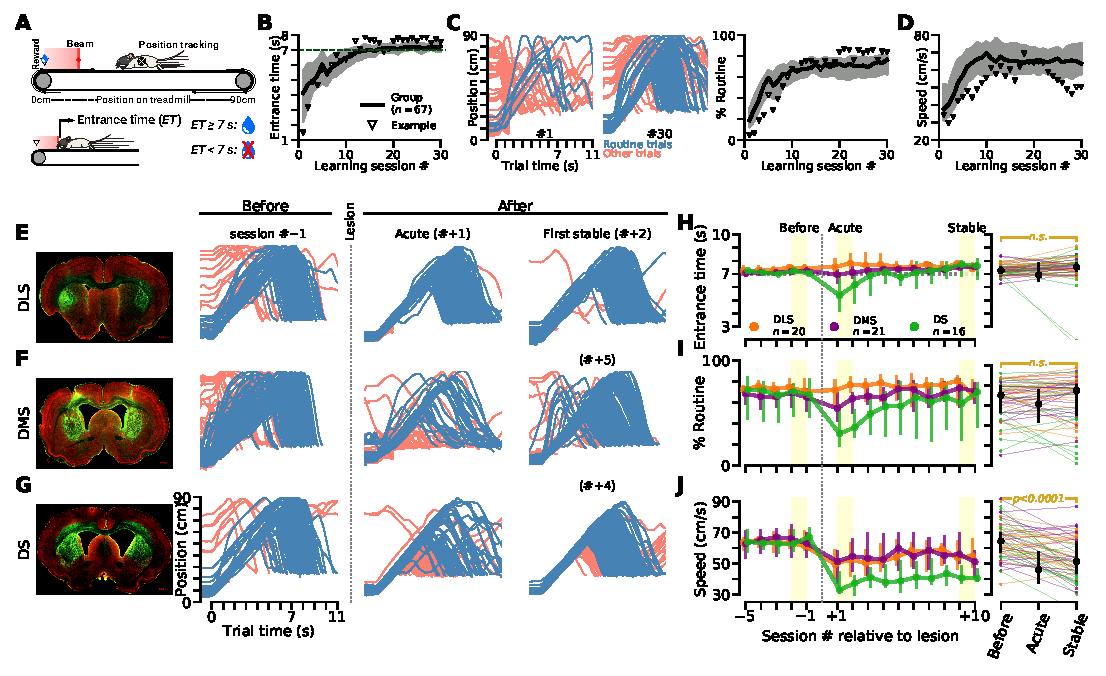
\includegraphics[width=\textwidth]{ch-lesion/figures/Task_Example_Group.pdf}
		\caption[The Striatum Energizes Motor Routines]
		{\textbf{The dorsal striatum is necessary to invigorate the running component of a motor routine.}
		\textbf{A)}
		Experimental apparatus and task rules, also refer to \autoref{fig:methods:taskRules}.
		\textbf{B)}
		Median \gls{et} across training sessions for all the rats trained in this task.
		Shaded area represents the 25th and 75th percentiles.
		Triangular markers in panels~B to~D indicate the performance for the example animal whose trajectories are shown in panel~C, left.
		\textbf{C)}
		Trajectories of an example animal on the treadmill, for all the trials performed in sessions \#1 and \#30 (\textit{left}).
		Percentage of trials during which animals performed the wait-and-run routine, across training sessions (\textit{right}).
		\textbf{D)}
		The running speed with which animals ran toward the reward area, across training sessions.
		\textbf{E-G)}
		Histology (\textit{left}, GFAP in green shows gliosis, red is NeuN) and trajectories of single animals with bilateral lesions of the striatum (\textit{right}) in sessions before and after the lesion.
		`\#'~indicates session number relative to the lesion operation.
		\textbf{H-J)}
		\textit{Left}: time course of the lesion effect on behavioral measures.
		\textit{Right}: statistical comparison of the group data before vs.\ (long) after the lesion (10000 resamples).
		Trajectory plots in panels~C, and~E--G are cut at the \gls{et}.
		}
		\label{fig:lesion:task}
	\end{center}
\end{figure}